\documentclass{beamer}
\usepackage[utf8]{inputenc}
\usepackage{graphicx}
\usepackage{hhline}
\usepackage{pdfpages}
\usepackage{xcolor}
\usepackage{makecell}
\usepackage[mode=buildnew]{standalone}
\usepackage{amsmath}
\usepackage{mathtools}
\usepackage{tikz}
\usepackage{environ}
\usepackage{fontawesome}
\usepackage{caption}
\usepackage[backend=bibtex,style=authoryear-comp,dashed=false,natbib=true]{biblatex}
\addbibresource{bibtex.bib}
% \setbeamertemplate{footline}[frame number]
\setbeamerfont{footnote}{size=\Tiny}
\setlength\bibitemsep{1.5\itemsep}
\graphicspath{{img/}}
\setbeamertemplate{navigation symbols}{}
\setbeamertemplate{page number in head/foot}{}
\setbeamertemplate{bibliography item}{}
\setbeamertemplate{caption}[numbered]
\setbeamercovered{transparent}
\renewcommand\refname{Bibliography}
\setbeamerfont{institute}{size=\small}
\usetheme{Frankfurt}
\usecolortheme{whale}
\DeclareMathOperator*{\argmax}{argmax} 
\DeclareCaptionFormat{myformat}{\fontsize{6}{6}\selectfont#1#2#3}
\captionsetup{format=myformat}
\captionsetup[figure]{labelfont={bf},name={Figure}}
\captionsetup[table]{labelfont={bf},name={Table}}
\renewcommand{\arraystretch}{1.1}

\newcommand{\customframefont}[1]{
	\setbeamertemplate{itemize/enumerate body begin}{#1}
	\setbeamertemplate{itemize/enumerate subbody begin}{#1}
}

\NewEnviron{framefont}[1]{
	\customframefont{#1} % for itemize/enumerate
	{#1 % For the text outside itemize/enumerate
		\BODY
	}
	\customframefont{\normalsize}
}

\setbeamertemplate{footline}{% 
	\hfill% 
	\usebeamercolor[fg]{page number in head/foot}% 
	\usebeamerfont{page number in head/foot}% 
	\insertframenumber%
	%\,/\,\inserttotalframenumber
	\kern1.2em\vskip4.5pt% 
}

\renewcommand\cellgape{\Gape[3pt]}
\definecolor{ao(english)}{rgb}{0.0, 0.5, 0.0}

\title{Mining Sentiments and Arguments in United
Nations Security Council (UNSC) Speeches}
\subtitle{"Exploring the UNSC political speech corpus"}
\author{Atreya Shankar, Juliane Hanel \\ Cognitive Systems (M.Sc.)}
\institute{PM: Mining Sentiments and Arguments \\ University of Potsdam, WiSe 19/20 \\ Prof. Dr. Manfred Stede}
\date{December 10. 2019}

\begin{document}
	\begin{frame}
		\maketitle
	\end{frame}
	
	\begin{frame}
		\frametitle{Table of Contents}
		\setbeamertemplate{enumerate items}[square]
		\begin{enumerate}
			\setlength\itemsep{1em}
			\item Introduction and Objectives
			\item Sentiment Analysis
			\item Argumentation Mining
			\item Outlook
			\item Bibliography
		\end{enumerate}
	\end{frame}
	
	\section{Introduction}
	\subsection{}
	\begin{framefont}{\footnotesize}
		\begin{frame}
			\frametitle{Introduction: UNSC Corpus}
			\vspace{-10pt}
			\begin{columns}
				\column{0.003\linewidth}
				\column{0.40\linewidth}
				\centering
				\begin{figure}
					\captionsetup{justification=centering}
					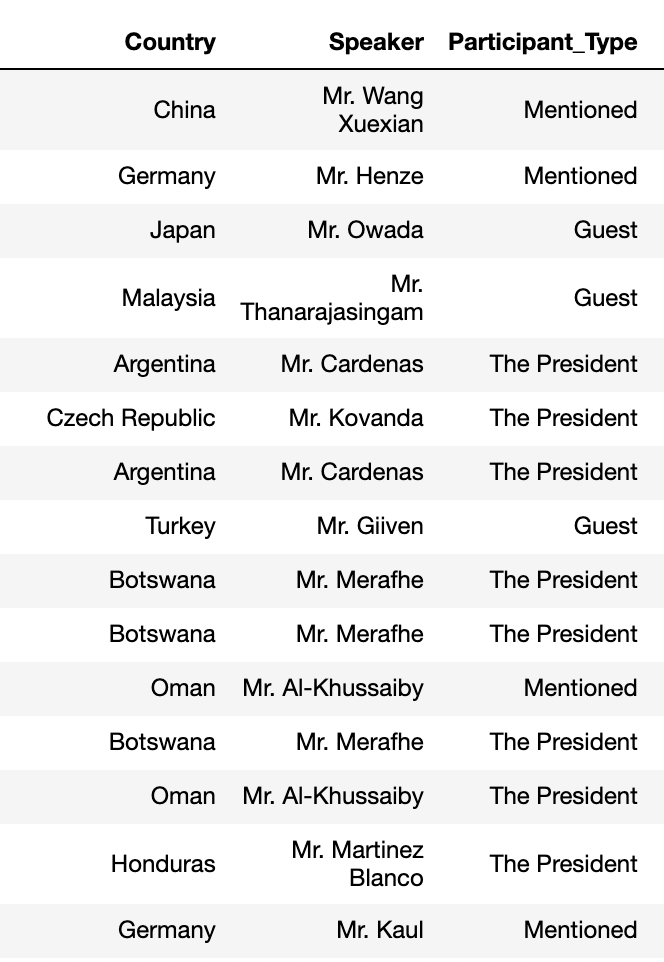
\includegraphics[trim={0.7cm 0cm 0.2cm 0.2cm},clip,width=4.4cm]{overview_dataset.png}
					\caption{Example structure of a UNSC speech}
				\end{figure}
				\column{0.60\linewidth}
				\begin{itemize}
					\setlength\itemsep{1.5em}
					\item The United Nations Security Council political speech corpus was released in \citet{schnfeld2019security}
					\item The corpus contains 65,393 speeches extracted from 4,958 UNSC meeting protocols 
					\item Metadata includes speech date, speaker, country, role in the UN and the participant type (president, mentioned, guest)
					%\parencite{}
					\item In addition, information about the topic and the number of types, tokens and sentences in the speech is provided
				\end{itemize}
			\end{columns}
		\end{frame}
	\end{framefont}

	\subsection{}
	\begin{framefont}{\footnotesize}
		\begin{frame}
		\vspace{5pt}
			\frametitle{Introduction: UNSC Descriptive Statistics}
			\begin{figure}
					\captionsetup{justification=centering}
					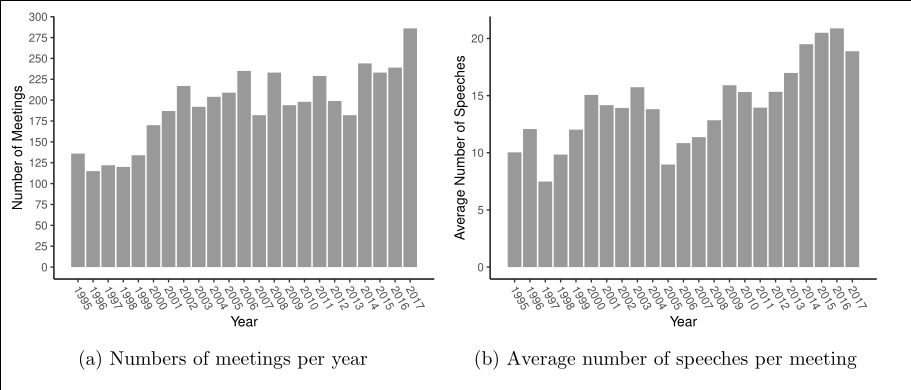
\includegraphics[trim={0.2cm 0cm 0cm 0.2cm},clip,width=8cm]{unsc_speeches_stats_1.png}
			\end{figure}
			\vspace{-5pt}
			\begin{figure}
					\captionsetup{justification=centering}
					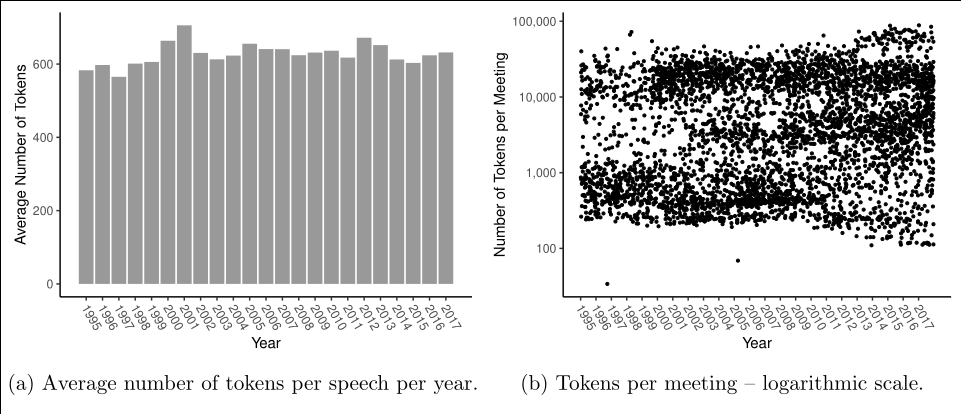
\includegraphics[trim={0.3cm 0cm 0cm 0.2cm},clip,width=8cm]{unsc_speeches_stats_2.png}
					\caption{Descriptive statistics of the UNSC corpus; adopted from \citet{schnfeld2019security}}
			\end{figure}
		\end{frame}
	\end{framefont}

	\subsection{}
	\begin{framefont}{\footnotesize}
		\begin{frame}
			\frametitle{Objectives}
			\begin{itemize}
				\setlength\itemsep{1.5em}
				\item \textbf{General objective:} Explore mining various components of the unannotated UNSC political speech corpus
				\item \textbf{Approach 1:} Using sentiment and subjectivity analysis
				\item \textbf{Approach 2:} Mining argumentation structure of speeches
				\item \textbf{Possible downstream task:} Using mined components to investigate whether given speech segments were spontaneous or planned
			\end{itemize}
		\end{frame}
	\end{framefont}

\section{Sentiment Analysis}
\subsection{}
\begin{framefont}{\footnotesize}
	\begin{frame}
		\frametitle{Methodologies: Sentiment Analysis I}
		\textbf{Methods:}
		\begin{itemize}
			\item Test multiple pre-developed sentiment analysis frameworks and compare their results on the UNSC corpus
			\item Expand the scope to subjectivity analysis
			\item Combine frameworks or improve them using domain-specific lexica
		\end{itemize}
		    \textbf{Possible research questions:}
		    \begin{itemize}
		        \item Does countries' sentiment change over time?
		        \item How diplomatic is the UNSC? - Do humanitarian crises affect the sentiment and subjectivity of council speeches?
		        \item Are sentiment and subjectivity cues for spontaneous and planned speech in the UNSC?
		    \end{itemize}
	\end{frame}
\end{framefont}

\subsection{}
\begin{framefont}{\footnotesize}
	\begin{frame}
		\frametitle{Methodologies: Sentiment Analysis II}
		
		\textbf{Used so far:}
		\begin{itemize}
			\setlength\itemsep{1.2em}
			\item \textit{Vader} and \textit{TextBlob} for comparative sentiment analysis ([-1,1] from negative over neutral to positive)
			\item \textit{TextBlob} for subjectivity analysis ([0,1] from objective to subjective)
			 

		\end{itemize}
		\\[10]
		\textbf{Sentiment scores differ among frameworks:}
				\begin{table}[]
        \begin{tabular}{|l|l|l|}
        \hline
        Vader Sentiment & TextBlob Sentiment & Subjectivity \\ \hhline{|=|=|=|}
        0.838                & 0.166                   & 0.425             \\ \hline
        
        \end{tabular}
        \\[3] %You can adjust how far below the table the text should appear
  \caption{Average sentiment/subjectivity scores for UNSC speeches in 1995}
  \\[3]
        \end{table}
	\end{frame}
\end{framefont}

\subsection{}
\begin{framefont}{\footnotesize}
	\begin{frame}
		\frametitle{Preliminary Results: Sentiment Analysis I}
		\vspace{20pt}
		\begin{enumerate}
		\setbeamertemplate{enumerate items}[square]
		    \item
		\begin{quotation}
		    The President: 
		    I thank the representative of Indonesia for the kind words he addressed to me.
		\end{quotation}
		\end{enumerate}
    \begin{table}[]
    \begin{tabular}{|l|l|l|l|l|l}
    \cline{1-5}
    Country & Speaker   & Vader\_Sent & Blob\_Sent & Subjectivity \\ \hhline{|=|=|=|=|=|}
    Italy   & Mr. Fulci     & 0.71           & 0.6                 & 0.9                    \\ \cline{1-5}
    \end{tabular}
    \caption{Example sentiment/subjectivity scores for short UNSC text}
    \end{table}

\begin{enumerate}
\setbeamertemplate{enumerate items}[square]
  \setcounter{enumi}{1}
    \item
\begin{quotation}
I apologize for speaking, but I wish to address the
statement [...]. It is not my habit to address such gratuitously
unpleasant comments [...], but I believe that for once I am obliged to do so. [...] But what does it really matter now? All this is trivial and has nothing whatever to do with the goal of this
meeting, [...].
\end{quotation}
\end{enumerate}
    \begin{table}[]
    \begin{tabular}{|l|l|l|l|l|l}
    \cline{1-5}
    Country & Speaker   & Vader\_Sent & Blob\_Sent & Subjectivity \\ \hhline{|=|=|=|=|=|}
    France   & Mr. Ladsous     & 0.98           & 0.12                 & 0.36                    \\ \cline{1-5}
    \end{tabular}
    \caption{Example sentiment/subjectivity scores for long UNSC text}
    \end{table}


	\end{frame}
\end{framefont}

\subsection{}
\begin{framefont}{\footnotesize}
	\begin{frame}
		\frametitle{Preliminary Results: Sentiment Analysis II}
		\begin{itemize}
			\setlength\itemsep{1.2em}
			\item Subjectivity classification reveals unusual scores for short spontaneous speeches (example: 0.9, average: 0.425)
			\item Does not catch the subjectivity of longer speeches
			\item \textbf{Assumption:} Formal or unusual vocabulary and syntax may affect the performance of the classifiers
			\item \textbf{Possible solutions:}
			\begin{itemize}
			    \item Improve pre-processing (e.g. identify common stop words)
			    \item  Use domain specific lexica (e.g. \citetitle{lexicoder}, \citetitle{subjective})
			    \item  Use a more sophisticated sentiment/subjectivity measure (e.g. pre-trained machine learning models)
			\end{itemize}
		\end{itemize}
	\end{frame}
\end{framefont}

\section{Argumentation Mining}
\subsection{}
\begin{framefont}{\footnotesize}
	\begin{frame}
		\frametitle{Methodologies: Argumentation Mining}
			\vspace{-10pt}
			\begin{figure}				       \captionsetup{justification=centering}
		   	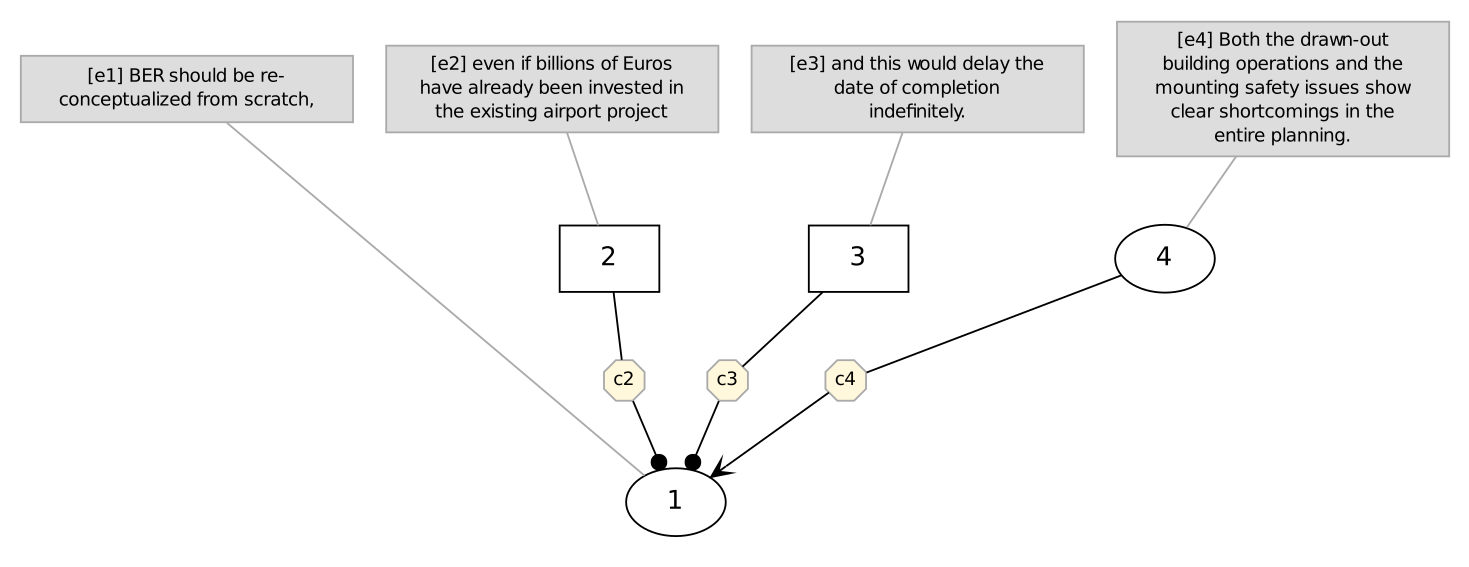
\includegraphics[trim={0cm 0cm 0cm 0cm},clip,width=8cm]{args_structure.png}
		   	\caption{Example of a complete argumentative structure of a short text \citep{peldszus2015annotated}}
			\end{figure}
		\begin{itemize}
			\setlength\itemsep{1.2em}
			\item Argumentation structure requires claims and premises
			\item Claims and premises are usually assembled into a tree structure
			\item Specify support/attack nature of claims and premises
		\end{itemize}
	\end{frame}
\end{framefont}

\subsection{}
\begin{framefont}{\footnotesize}
	\begin{frame}
		\frametitle{Methodologies: Potash et al. 2016}
			\vspace{2pt}
			\begin{figure}				       \captionsetup{justification=centering}
		   	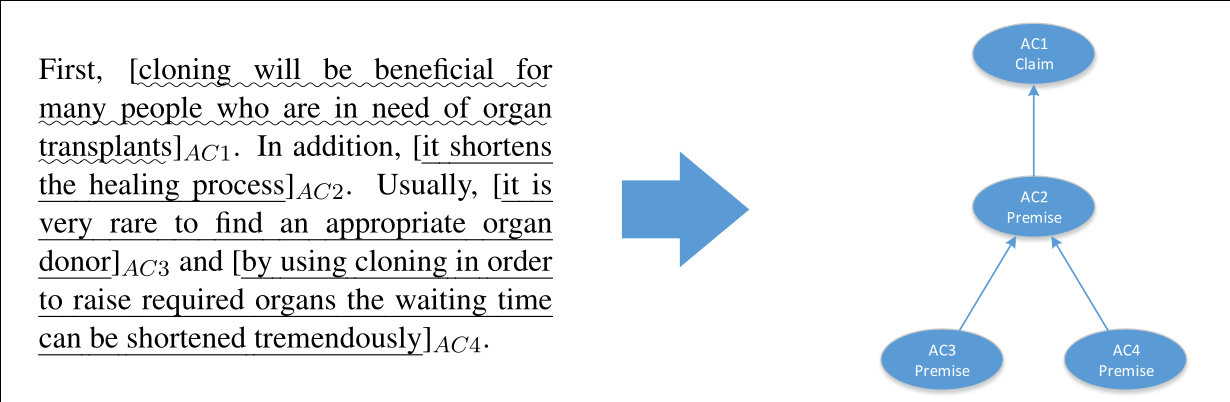
\includegraphics[trim={0.5cm 0cm 0cm 0.5cm},clip,width=8cm]{potash_args.png}
		   	\caption{Simplified argumentation structure in \citet{potash2016heres}}
			\end{figure}
			\begin{figure}				       \captionsetup{justification=centering}
		   	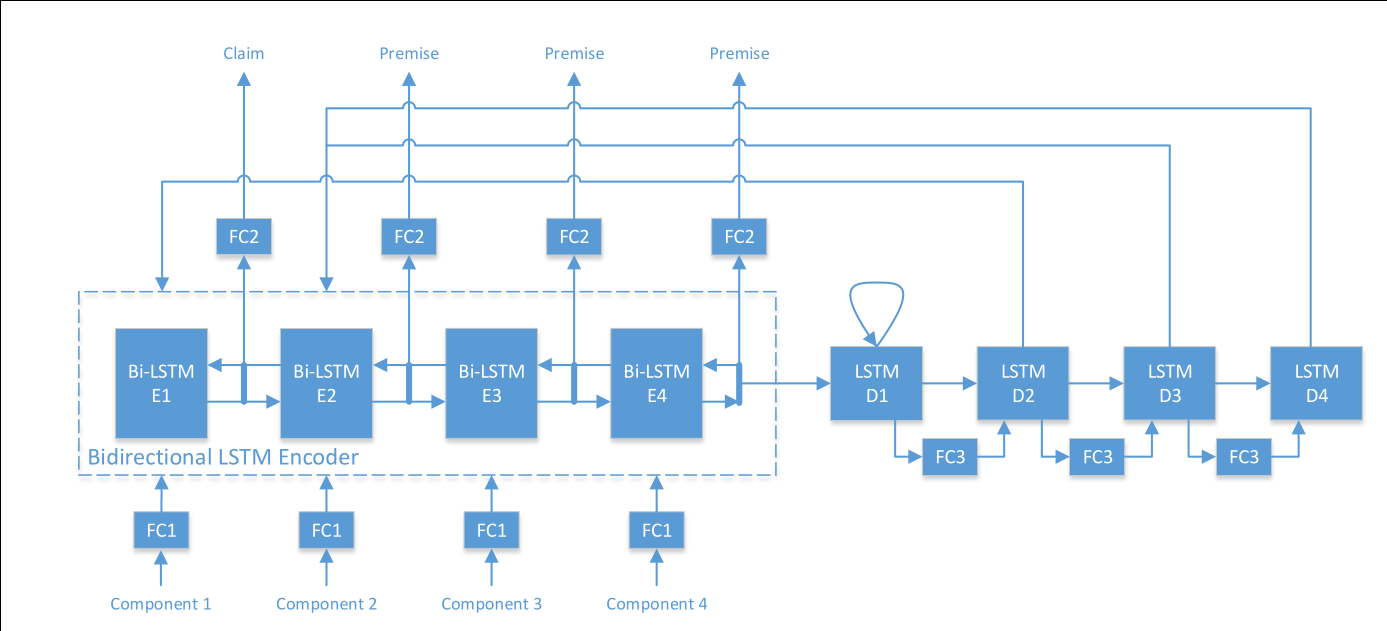
\includegraphics[trim={0.5cm 0cm 0cm 1.6cm},clip,width=8cm]{potash_model.png}
		   	\caption{Joint self-attention pointer network developed in \citet{potash2016heres}}
			\end{figure}
	\end{frame}
\end{framefont}

\subsection{}
\begin{framefont}{\footnotesize}
	\begin{frame}
	\frametitle{Methodologies: Application on UNSC dataset I}
	\begin{enumerate}
	    \setlength\itemsep{1.5em}
		\setbeamertemplate{enumerate items}[square]
	    \item Joint pointer neural network \citep{potash2016heres}
	    \begin{itemize}
	    	\setlength\itemsep{1em}
	        \item State-of-the-art results, but excludes attack/support
	        \item Assumes claim/premise candidates are provided in a span
	        \item \textbf{Extra pipeline needed to identify argument candidates}
	    \end{itemize}
	    \item Training dataset
	    \begin{itemize}
	    	\setlength\itemsep{1em}
	    	\item Microtext corpus \citep{peldszus2015annotated} \\
	    	$\Longrightarrow$ short texts and lack of domain knowledge
	        \item \textbf{US election debate corpus \citep{haddadan-etal-2019-yes}} $\Longrightarrow$ new corpus in political domain, but occasional inaccurate annotations\footnote{\url{https://github.com/ElecDeb60To16/Dataset/issues/2}}
	        \item \textbf{Persuasive essay corpus \citep{stab2017parsing}} \\
	        $\Longrightarrow$ medium length formal essays with accurate annotations
	    \end{itemize}
	\end{enumerate}
	\end{frame}
\end{framefont}

\subsection{}
\begin{framefont}{\footnotesize}
	\begin{frame}
	\frametitle{Methodologies: Application on UNSC dataset II}
	\begin{align}
	\text{Let } \mathbf{X} &= \left[The, world, is, nice, thus, I, am, happy\right] \\[5pt]
	\mathbf{Y_1} &= f_1(\mathbf{X}) = \left[1, 1, 1, 1, 0, 1, 1, 1\right] \\[5pt]
	\mathbf{Y_2} &= f_2(\mathbf{X}) = \left[-1, -1, -1, -1, 0, 1, 1, 1\right]
	\end{align}
	\begin{itemize}
	    \setlength{\itemsep}{1em}
	    \item Identifying argument candidates corresponds to a \textit{seq2seq} task
	    \item Input $\mathbf{X}$ can be transformed to arbitrary argument candidates $\mathbf{Y_1}$
	    \item Input $\mathbf{X}$ can be jointly transformed to specific argument candidates $\mathbf{Y_2}$, or alternatively to higher order argument structures such as a tree
	    \item Leverage on recent developments in \textit{seq2seq} pipelines \\
	    $\Longrightarrow$ Transformers, BERT pre-trained encoders
	\end{itemize}
	\end{frame}
\end{framefont}

\section{Outlook}
\subsection{}
\begin{framefont}{\footnotesize}
	\begin{frame}
		\frametitle{Outlook}
		\begin{enumerate}
		\setbeamertemplate{enumerate items}[square]
			\setlength\itemsep{1.2em}
			\item Develop more consistent sentiment analysis tools for the UNSC corpus
			\item Apply trained argumentation classifier (single or multi-task) onto corpus
			\item Develop an evaluation strategy for results:
			\begin{itemize}
			    \item Crowd sourcing to rate automatic annotations
			    \item Manual annotation of representative subsets of corpus
			\end{itemize}
		\end{enumerate}
	\end{frame}
\end{framefont}

\begin{frame}[allowframebreaks]
	\frametitle{Bibliography}
	\nocite{*}
	\printbibliography[title = {Bibliography}]
\end{frame}

\end{document}KK